\ylDisplay{Varras} % Ülesande nimi
{Tundmatu autor} % Autor
{lõppvoor} % Voor
{2015} % Aasta
{P 5} % Ülesande nr.
{3} % Raskustase
{
% Teema: Mehaanika

\ifStatement
Varras $AC$ võib pöörelda ümber punkti $B$ ja varras $DF$ ümber punkti $F$. Varda $AC$ otsad on niitidega kinnitatud varda $DF$ külge. On teada, et$ AB = 2a$,$ BC = a$ ja $DF = 4a$. Kui suured on niitides $AD$ ja $CE$ mõjuvad jõud? Varda $DF$ mass $m = 6$ $kg$ ning on jaotunud ühtlaselt üle kogu varda. Varda $AC$ massi ei ole tarvis arvestada.
\begin{center}
	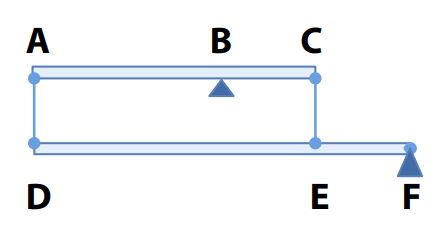
\includegraphics[width=0.5\linewidth]{2015-v3p-05-yl.PNG}
\end{center}
\fi

\ifHint
Niidile $EC$ mõjuv jõud on 2 korda suurem niidile $AD$ mõjuvast jõust ning need peavad olema tasakaalus vardale $DF$ tema keskpunktis mõjuva raskusjõuga.
\fi

\ifSolution
Kuna jõuõlg $AB = 2BC$ ja varda $AC$ massi pole tarvis arvestada, on niidile $AD$ mõjuv jõud $F_1$, mis on suunatud üles ja punktis $E$ jõud $2F_1$, mis ka on suunatud üles. Varda keskpunktis mõjub vardale jõud $mg$, mis on suunatud alla. Sellest lähtuvalt saab kirjutada jõumomentide tasakaalu võrrandi. 
\begin{center}
$F_1 4a + 2F_1 a - mg2a = 0$, Siit, $F_1 = \frac{mg}{3}$. 
\end{center}
Seega vasakus niidis mõjub jõud $20 N$ ja paremas niidis $40 N$.
\fi
}